\documentclass{article}
\usepackage[paperwidth=320mm,paperheight=180mm,margin=0pt]{geometry}
\usepackage[T1]{fontenc}
\usepackage{lmodern}
\usepackage{xcolor}
\usepackage{tikz}
\usetikzlibrary{positioning,arrows.meta,calc}
\renewcommand{\familydefault}{\sfdefault}
\pagestyle{empty}
\setlength{\parindent}{0pt}
% Shared palette. The category colours match the terminal report exactly,
% so a judge watching the demo sees the same colour mean the same thing.
\definecolor{night}{HTML}{0E1116}
\definecolor{panel}{HTML}{161B22}
\definecolor{hair}{HTML}{30363D}
\definecolor{ink}{HTML}{E6EDF3}
\definecolor{muted}{HTML}{8B949E}
\definecolor{regression}{HTML}{F85149}
\definecolor{flaky}{HTML}{D29922}
\definecolor{infra}{HTML}{58A6FF}
\definecolor{dependency}{HTML}{BC8CFF}
\definecolor{config}{HTML}{39C5CF}
\definecolor{good}{HTML}{3FB950}


\begin{document}
\noindent%
% The page is exactly 32cm x 18cm; draw on it directly rather than using
% remember-picture/overlay, which needs a second pass to place anything.
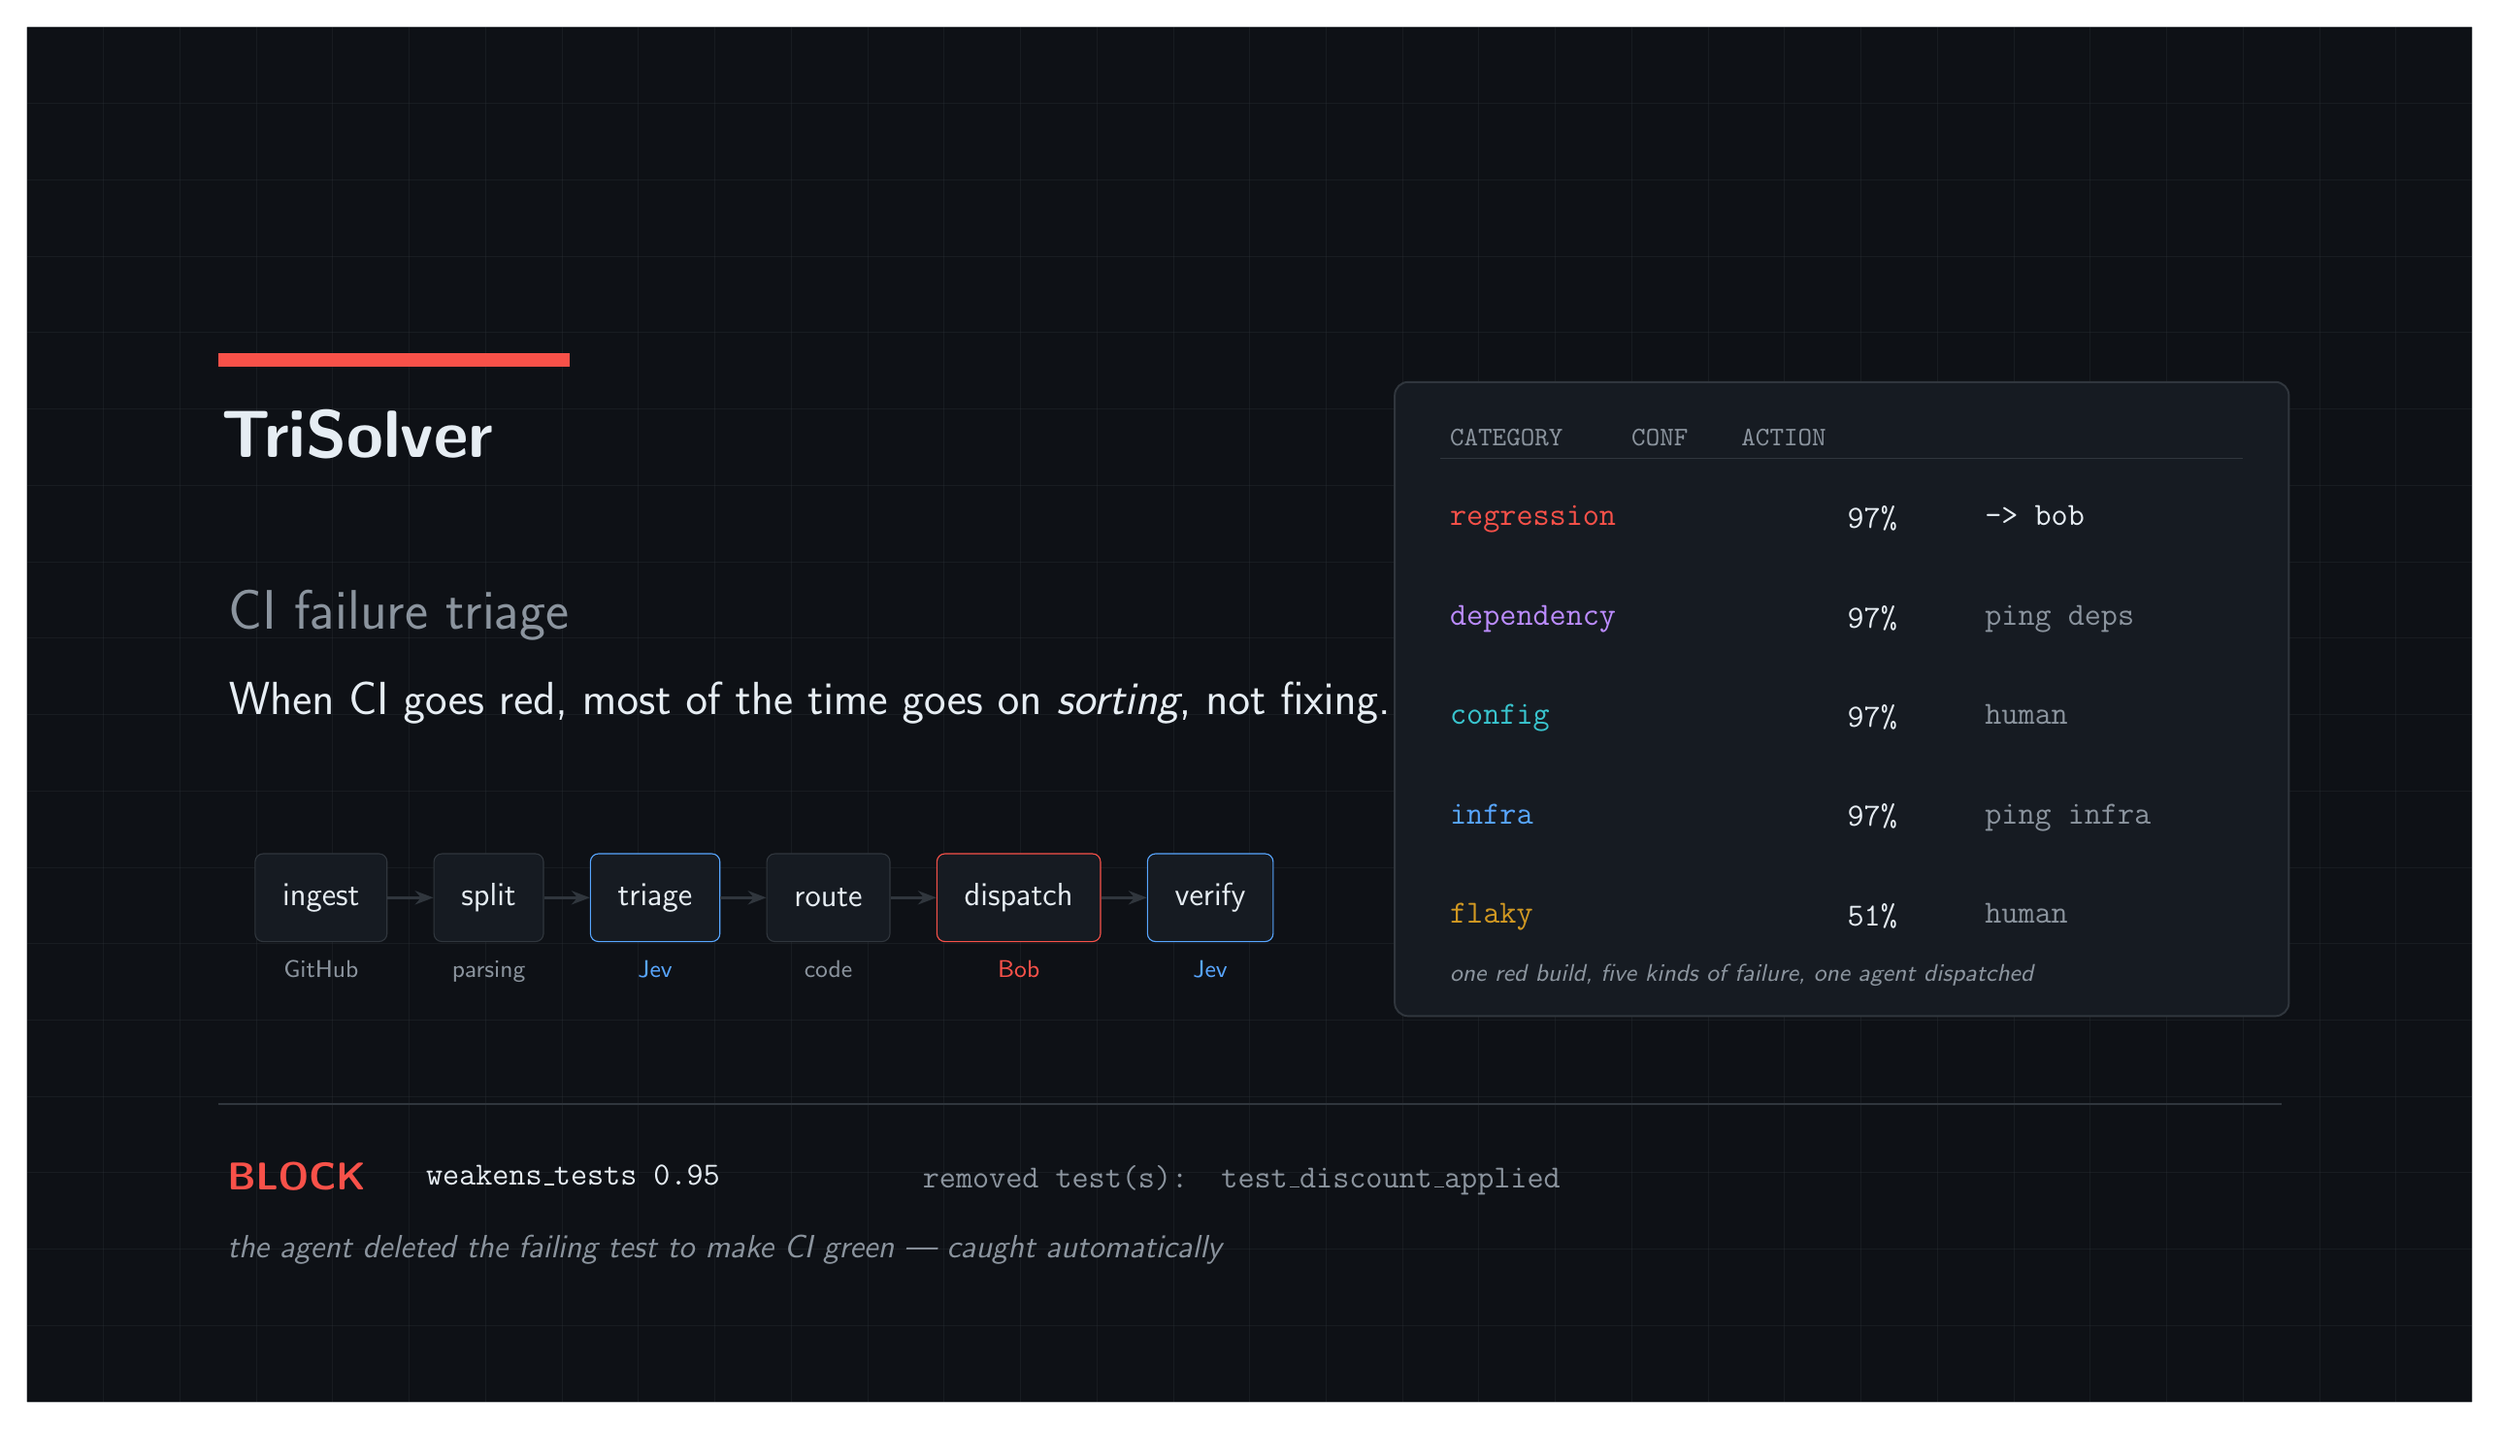
\begin{tikzpicture}[x=1cm,y=1cm]
  \useasboundingbox (0,0) rectangle (32,18);
  \fill[night] (0,0) rectangle (32,18);

  % faint grid for texture
  \foreach \x in {0,1,...,32}{\draw[hair,opacity=0.30,line width=0.2pt] (\x,0) -- (\x,18);}
  \foreach \y in {0,1,...,18}{\draw[hair,opacity=0.30,line width=0.2pt] (0,\y) -- (32,\y);}

  % accent rule
  \fill[regression] (2.5,13.55) rectangle (7.1,13.73);

  \node[anchor=north west, ink, font=\fontsize{78}{82}\bfseries]
    at (2.42,13.1) {TriSolver};
  \node[anchor=north west, muted, font=\fontsize{22}{26}\selectfont]
    at (2.52,10.75) {CI failure triage};
  \node[anchor=north west, ink, font=\fontsize{16}{23}\selectfont, text width=18cm]
    at (2.52,9.55)
    {When CI goes red, most of the time goes on \textit{sorting}, not fixing.};

  % pipeline
  \begin{scope}[
      chip/.style={draw=hair, fill=panel, rounded corners=3pt,
                   minimum height=1.15cm, inner xsep=0.36cm,
                   font=\fontsize{13}{13}\selectfont, text=ink},
      lbl/.style={font=\fontsize{9}{10}\selectfont, text=muted, inner sep=1.5pt},
      arr/.style={-{Stealth[length=2.4mm]}, hair, line width=1pt}]
    \node[chip]                                     (i) at (3.85,6.6) {ingest};
    \node[chip, right=0.60cm of i]                  (s) {split};
    \node[chip, right=0.60cm of s, draw=infra]      (t) {triage};
    \node[chip, right=0.60cm of t]                  (r) {route};
    \node[chip, right=0.60cm of r, draw=regression] (d) {dispatch};
    \node[chip, right=0.60cm of d, draw=infra]      (v) {verify};
    \foreach \a/\b in {i/s,s/t,t/r,r/d,d/v}{\draw[arr] (\a) -- (\b);}
    \node[lbl, below=0.18cm of i] {GitHub};
    \node[lbl, below=0.18cm of s] {parsing};
    \node[lbl, below=0.18cm of t, text=infra] {Jev};
    \node[lbl, below=0.18cm of r] {code};
    \node[lbl, below=0.18cm of d, text=regression] {Bob};
    \node[lbl, below=0.18cm of v, text=infra] {Jev};
  \end{scope}

  % right panel: the real board, so the cover shows the product
  \fill[panel, rounded corners=5pt] (17.9,5.05) rectangle (29.6,13.35);
  \draw[hair, rounded corners=5pt, line width=0.7pt] (17.9,5.05) rectangle (29.6,13.35);
  \node[anchor=north west, font=\fontsize{10}{10}\ttfamily, text=muted] at (18.5,12.85)
    {CATEGORY\hspace{0.9cm}CONF\hspace{0.7cm}ACTION};
  \draw[hair, line width=0.5pt] (18.5,12.35) -- (29.0,12.35);
  \begin{scope}[
      cat/.style={anchor=north west, font=\fontsize{11.5}{11.5}\ttfamily},
      num/.style={anchor=north east, font=\fontsize{11.5}{11.5}\ttfamily, text=ink},
      act/.style={anchor=north west, font=\fontsize{11.5}{11.5}\ttfamily, text=muted}]
    \node[cat, text=regression] at (18.5,11.85) {regression};
      \node[num] at (24.6,11.85) {97\%}; \node[act, text=ink] at (25.5,11.85) {-> bob};
    \node[cat, text=dependency] at (18.5,10.55) {dependency};
      \node[num] at (24.6,10.55) {97\%}; \node[act] at (25.5,10.55) {ping deps};
    \node[cat, text=config]     at (18.5,9.25)  {config};
      \node[num] at (24.6,9.25)  {97\%}; \node[act] at (25.5,9.25)  {human};
    \node[cat, text=infra]      at (18.5,7.95)  {infra};
      \node[num] at (24.6,7.95)  {97\%}; \node[act] at (25.5,7.95)  {ping infra};
    \node[cat, text=flaky]      at (18.5,6.65)  {flaky};
      \node[num] at (24.6,6.65)  {51\%}; \node[act] at (25.5,6.65)  {human};
  \end{scope}
  \node[anchor=north west, font=\fontsize{9.5}{9.5}\itshape, text=muted] at (18.5,5.85)
    {one red build, five kinds of failure, one agent dispatched};

  % the hook
  \draw[hair, line width=0.7pt] (2.5,3.9) -- (29.5,3.9);
  \node[anchor=north west, font=\fontsize{15}{15}\bfseries, text=regression] at (2.5,3.25) {BLOCK};
  \node[anchor=north west, font=\fontsize{13}{13}\ttfamily, text=ink]        at (5.1,3.22) {weakens\_tests 0.95};
  \node[anchor=north west, font=\fontsize{13}{13}\ttfamily, text=muted]      at (11.6,3.22) {removed test(s): test\_discount\_applied};
  \node[anchor=north west, font=\fontsize{13}{18}\itshape, text=muted]       at (2.5,2.3)
    {the agent deleted the failing test to make CI green --- caught automatically};
\end{tikzpicture}
\end{document}
